\section{Considerações Iniciais}

Como apresentado no Capítulo~\ref{chapter:adm_kdm} o metamodelo KDM é capaz de agrupar diferentes visões/artefatos de um determinado sistema em uma única instância, bem como representar todas as dependências entre tais visões/artefatos. Usualmente, o que é encontrado na literatura (colocar refs)\change{Colocar as refs achadas...} durante o desenvolvimento e manutenção de software seguindo as diretrizes e passos da abordagem MDE, é que o software geralmente é modelado e representado utilizando diferentes instâncias de metamodelos para representar as visões e todos os artefatos de um sistema. Em outras palavras, geralmente existem metamodelos para abstrair e representar o código-fonte, metamodelos para representar e abstrair o banco de dados, metamodelos para representar e abstrair a arquitetura do sistema, etc. 

Uma premissa fundamental é manter todas as instâncias dos metamodelos que representam as visões/artefatos sincronizados durante todo o processo de modernização do software. Dessa forma, quando as visões/artefatos representados em nível de modelos são alterados, é de extrema importância realizar um conjunto de propagação de mudança por todas as visões/artefatos para mantê-los atualizados e sincronizados, espelhando assim, a alteração em todas as visões/artefatos do software. Usualmente, como apresentado nos Capítulo~\ref{chapter:fundamentacao_teorica}, Seção~\ref{sec:refatoracao} e Capítulo~\ref{chapter:catalogo_refactoring_KDM} essas alterações podem ser realizadas por meio de refatorações, as quais são atividades centrais durante o processo de modernização (ref)\change{aqui tbm}. Porém, quando um software é representado utilizando diferentes instâncias de metamodelos, um acidente comum que pode ocorrer durante a atividade de refatoração é a dessincronização dessas instâncias, fazendo com que as visões/artefatos que representam o sistema fiquem inconsistente após a atividade de refatoração. Uma das forma de resolver esse problema é aplicar técnicas de propagação de mudança, cujo objetivo é identificar e atualizar todas as instâncias dependentes dos elementos que foram refatorados. No entanto, a maioria das propostas de propagação de mudança foram desenvolvidas para propagarem mudanças em diferentes metamodelos, além disso, usualmente tais metamodelos são de diferentes fornecedores dificultando o entendimento e a programação de mudança (ref). 
Diante deste contexto, neste capítulo é apresentado uma abordagem para realizar a propagação de mudança e preservação de comportamento após a aplicação de refatorações no metamodelo KDM. Utilizando a abordagem aqui definida, modernizadores podem se concentrar apenas no desenvolvimento das refatorações ou reutiliza-las por meio do metamodelo SRM (ver Capítulo~\ref{chapter:Toward_a_Refactoring_Metamodel_for_KDM}), sem terem que se preocuparem com a propagação de mudanças para outras visões do metamodelo KDM. 

É importante destacar que o fluxo da abordagem inicia-se considerando que o modernizador almeja aplicar um conjunto de refatorações em um sistema que está já representado por meio de uma instância do metamodelo KDM. Essa instância do metamodelo KDM deve estar o mais completo possível, ou seja, represente todas as visões/artefatos do sistema, desde o código-fonte até os elementos arquiteturais do sistema. Após o modernizador aplicar uma determinada refatoração, a abordagem, a qual contêm três principais passos, efetivamente é iniciada. 

De forma resumida pode-se descrever os três passos da abordagem da seguinte forma. O primeiro passo da abordagem realiza uma comparação (do inglês - \textit{diff}) entre a instância refatorada do metamodelo KDM com a instância do metamodelo KDM original, ou seja, a instância do metamodelo KDM antes do modernizador aplicar a refatoração. Como resultado, esse passo cria uma lista que contêm todas as instâncias das metaclasses do KDM que sofreram uma modificação durante a refatoração quando comparado com a instância do KDM original. Em seguida, o segundo passo utiliza como entrada a lista gerada para ser utilizada como parâmetro para um algoritmo de mineração e identificação de dependências. Esse algoritmo tem como objetivo identificar todas as instâncias das metaclasses do KDM que possuem dependência com as metaclasses refatoradas. Como resultado, esse algoritmo também cria uma lista, a qual é utilizada no terceiro passo. O terceiro passo utiliza a lista criada pelo algoritmo para realizar um conjunto de transformações em nível de modelo. Tais transformações foram pré-definidas e representam a propagação de mudança por todas as visões do KDM. É importante destacar que a abordagem foi implementada com a preocupação de ser uma forma genérica e desacoplada. Assim, a abordagem pode ser aplicada em um grande conjunto de refatorações fazendo com que o modernizador não se preocupe com a propagação. 

As demais seções deste capítulo estão organizadas da seguinte forma:\change{terminar aqui. Deve colocar todas as seções bem escritas.}


\section{A Abordagem KDM-SInc}\label{sec:kdm_sinc}

Nessa seção a abordagem denominada KDM-SInc é apresentada. Essa abordagem têm como objetivo propagar mudanças por todas as visões/artefatos do metamodelo KDM para mantê-lo atualizado e sincronizado após a aplicação de uma refatoração. A intenção é criar uma abordagem que mantenha uma determinada instância do metamodelo KDM consistênte e sincronizada entre todas as visões/artefatos do metamodelo KDM após a aplicação de uma determinada refatoração. 

Na Figura~\ref{fig:kdm_sinc} é apresentado uma visão geral da abordagem KDM-SInc. Como pode ser observado a abordagem KDM-SInc contêm três principais passos, os quais estão contidos em um módulo de propagação (caixa cinza). Antes de iniciar o módulo de propagação uma atividade de refatoração deve ser realizada como apresentado na Figura~\ref{fig:kdm_sinc} lado esquerdo caixa branca. A atividade de refatoração esta fora do escopo da abordagem KDM-SInc, assim, é de responsabilidade do engenheiro de modernização criar e/ou reutilizar refatoração para o metamodelo KDM e aplica-la em uma instância do metamodelo KDM. A única restrição da abordagem KDM-SInc é que duas versões da instância do metamodelo KDM seja utilizada como entrada para a abordagem - uma versão que representa a instância do metamodelo KDM antes da aplicação das refatorações (instância original) e outra versão que representa uma instância do metamodelo KDM após a aplicação de \textit{n} refatorações (instância refatorada).

\begin{figure}[h]
	\centering
	% Requires \usepackage{graphicx}
	\caption{Visão Geral da Abordagem KDM-SInc.}
	\label{fig:kdm_sinc}
	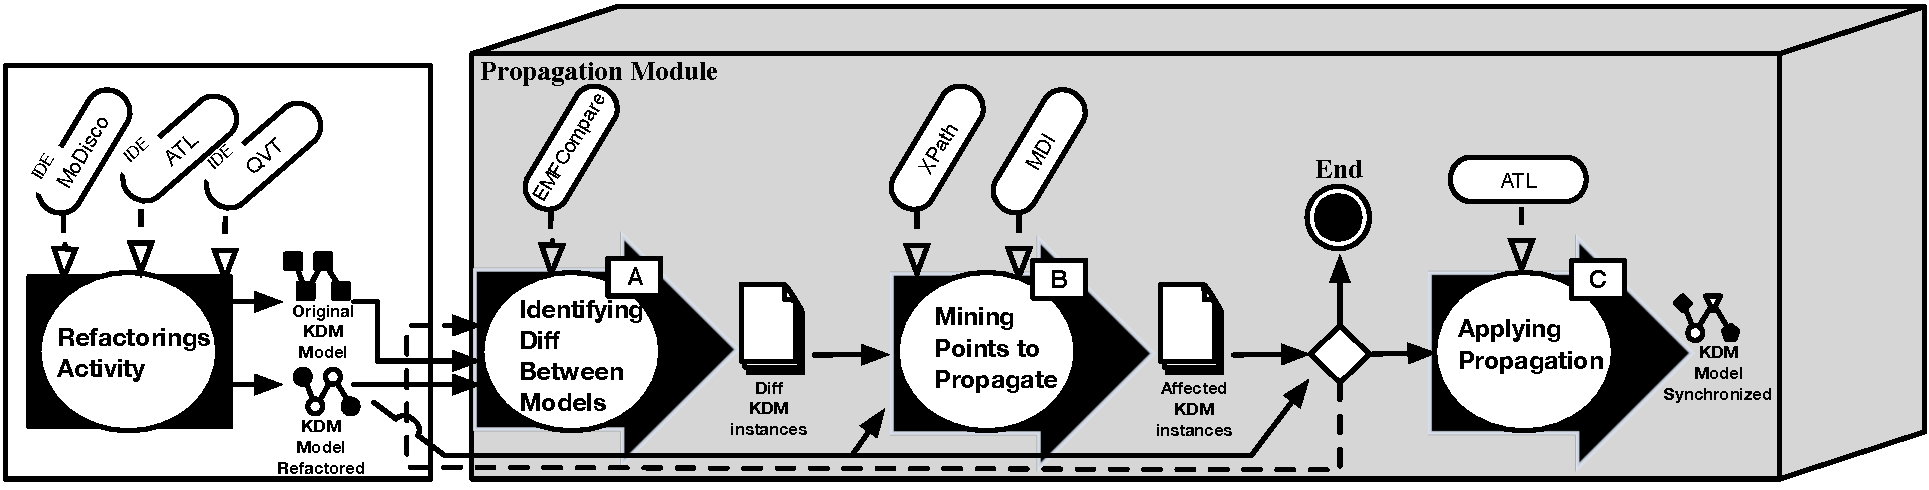
\includegraphics[scale=0.5]{images/ApproachLifeCicle2}
	\fautor
\end{figure}

Após a aplicação de um conjunto de refatorações o passo [A] pode ser iniciado. Nesse passo uma comparação (\textit{diff}) entre a instância original e a instância refatorada é realizada. Como resultado desse passo uma lista é crida. Essa lista contêm todas as instâncias das metaclasses do KDM que sofreram alguma modificação durante a refatoração quando comparado com a instância do KDM original. Além disso, essa lista também especifica qual(is) foi(ram) a(s) modificação(ões) realizada(s). Por exemplo, essa se na versão refatorada uma nova instância da metaclasse \texttt{ClassUnit} foi adicionada a lista irá conter duas informações: (\textit{i}) a instância da metaclasse \texttt{ClassUnit} e (\textit{ii}) qual operação foi realizada, nesse exemplo \texttt{add} \texttt{ClassUnit}.

Em seguida o passo [B] é iniciado, o qual identifica todas as metaclasses que precisam ser sincronizadas/atualizadas após a aplicação da refatoração. Nesse passo utiliza o algoritmo de busca em profundidade (do inglês - \textit{Depth-First Search} - DFS). Para a abordagem KDM-SInc algoritmo DFS foi alterado para utilizar como entrada a lista criada no passo [A]. Além disso, o algoritmo DFS também utiliza como entrada a instância refatorado do KDM. Utilizando a instância refatorado o algoritmo DFS identifica e cria uma lista contendo todas as metaclasses que possuem dependência com as metaclasses que efetivamente foram refatoradas.

Posteriormente o passo [C] pode ser iniciado. Esse passo denominado \aspas{Aplicar Propagação} realiza todas as mudanças na instância do metamodelo KDM. Como entrada esse passo utiliza todas as metaclasses que possuem dependência com as metaclasses que foram refatoradas (lista criada no passo [B]). Após o término do passo [C] todas as visões/artefatos da instância do metamodelo KDM estão sincronizadas e consistentes.

É importante salientar que os três passos da abordagem KDM-SInc são executados várias vezes até que não hava mais elementos que precisem ser atualizados/sincronizados. Esse ciclo é necessário uma vez que uma determinada instância do metamodelo KDM pode ainda exigir propagações em outros artefatos/visões, por isso, cada ciclo da abordagem KDM-SInc se concentra apenas no próximo nível de propagação. A condição de parada da abordagem KDM-SInc é quando o algoritmo, definido no passo [B], retornar uma lista vazia, indicando que não há mais elementos que precisam ser modificados.

Para auxiliar a elaboração do passo [A] o \textit{framework} EMFCompare\footnote{https://www.eclipse.org/emf/compare/} foi estendido para comparar instâncias do metamodelo KDM. O passo [B] é tecnicamente apoiado por um motor de busca cuja parte central é o algoritmo DFS juntamente com um conjunto de OCL \textit{queries} que são executadas em uma instância do metamodelo KDM. Finalmente, o passo [C] é apoiado por um motor de propagação, o qual utiliza um conjunto de transformações pré-definidas em ATL para executar as propagações. Todas as propagações foram definidas com base nas operações atômicas (\texttt{add}, \texttt{delete} e \texttt{change}) apresentadas no Capítulo X \change{Mudar aqui}. Dessa forma, quando um conjunto de refatorações são executadas propagações bem definidas podem ser executadas no contexto do metamodelo KDM. Maiores detalhes sobre cada passo é apresentado nas próximas seções.

\subsection{Identificando \textit{Diff} entre Instâncias do Metamodelo KDM}\label{sec:diff_entre_kdm}

Nessa seção o primeiro passo da abordagem KDM-SInc é apresentado. Como já salientado o primeiro passo da abordagem KDM-SInc utiliza o \textit{framework} EMFCompare. Esse \textit{framework} foi escolhido pois o mesmo pode ser facilmente adaptado e estendido. Especificadamente o passo [A] da abordagem KDM-SInc realizada três sub-passos: (\textit{i}) \textit{matching}, (\textit{ii}) \textit{diffing} e (\textit{iii}) análise dos \textit{diffs} como apresentado na Figura~\ref{fig:diff_emf_compare}. 

\begin{figure}[h]
	\centering
	% Requires \usepackage{graphicx}
	\caption{Visão Geral da Execução do Primeiro Passo da Abordagem KDM-SInc.}
	\label{fig:diff_emf_compare}
	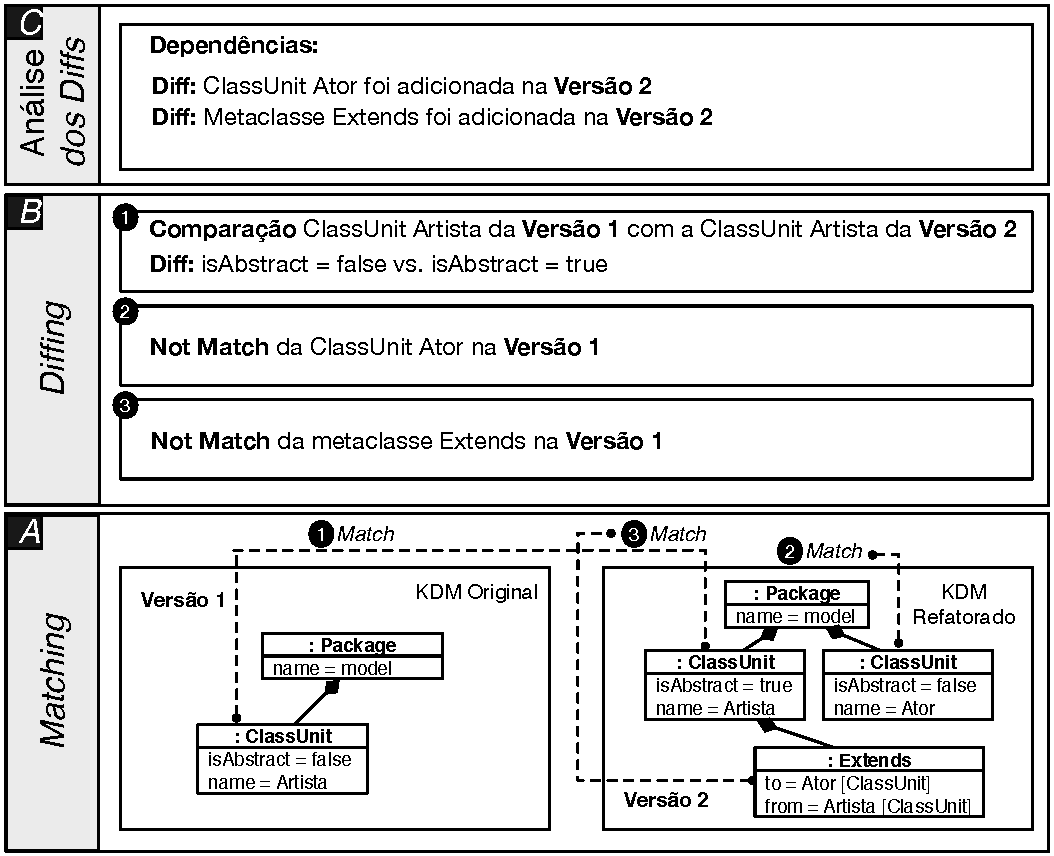
\includegraphics[scale=0.8]{images/matching_diffing_analise_2}
	\fautor
\end{figure}

Com pode ser observado na Figura~\ref{fig:diff_emf_compare} o primeiro sub-passo, \textit{matching}, necessita de duas instâncias do metamodelo KDM - uma instância original (KDM original no lado esquerdo) denominada \textbf{versão 1} na Figura~\ref{fig:diff_emf_compare} e uma instância refatorada (KDM refatorado no lado direito) \textbf{versão 2} na Figura~\ref{fig:diff_emf_compare}. Dado as duas instâncias do metamodelo KDM, os correspondentes elementos nas duas versões do metamodelo KDM são identificados. Os correspondentes elementos são identificados por meio de identificadores únicos tais como XMI IDs. Por exemplo, na Figura~\ref{fig:diff_emf_compare} pode-se observar que a instância da metaclasse \texttt{ClassUnit} Artista apresentada na \textbf{versão 1} corresponde a instância da metaclasse \texttt{ClassUnit} Artista na \textbf{versão 2}. Para as instâncias das metaclasses \texttt{ClassUnit} Ator e \texttt{Extends} na \textbf{versão 2}, no entanto, nenhum elemento correspondente foi identificado na \textbf{versão 1}.

No segundo sub-passo, \textit{Diffing}, todos os correspondentes elementos identificados são examinados para identificar diferenças em seus meta-atributos. Para cada diferença identificada um objeto \textit{diff} é criado, o qual descreve com precisão cada diferença entre os correspondentes elementos. Por exemplo, ainda considerando a Figura~\ref{fig:diff_emf_compare}, quando a instância da metaclasse \texttt{ClassUnit} Artista da \textbf{versão 1} e \textbf{versão 2} são examinadas é possível observar que o meta-atributo \texttt{isAbstract} possui o valor \textit{false} na \textbf{versão 1}, enquanto que na \textbf{versão 2} o mesmo meta-atributo o valor é \textit{true}. Instâncias de metaclasses que não contêm elementos correspondentes em ambas as versões são consideradas adicionadas ou deletadas - a operação é identificada dependendo da direção, por exemplo, se uma instância de uma metaclasse apenas existe do lado direito essa instância foi adicionada, por outro lado, se uma instância apenas existe do lado esquerdo essa instância foi deletada. Neste contexto, na Figura~\ref{fig:diff_emf_compare} é possível identificar que duas instâncias foram adicionadas - uma instância da metaclasse \texttt{ClassUnit} denominada Ator e uma instancia da metaclasse \texttt{Extends}.

\section{Considerações Finais}
